%% ----------------------------------------------------------------
%% VideoPlayer.tex
%% ---------------------------------------------------------------- 
\chapter{Video Player} 
\label{Chapter:Video Player}

\todo{Work out sectioning, probably each plugin needs a new chapter, Motivation, work, conclusion}

Specific improvements to \gls{Videogular} were made up three main sections, accessibility, compatibility and scrub bar plugin creation. Each were conducted independently and the open source contributions accepted readily back into the main \gls{Videogular} project.

The main goals for this part of the project were to:
\begin{itemize}
\item investigate \gls{Videogular} to allow for its use within the new version of Synote
\item improve the accessibility of \gls{Videogular} to allow for its use by users with less than normal interface  devices
\item ensure that \gls{Videogular} was as compatible on as many devices as possible
\item add the ability to mark locations on the scrub bar
\item produce a plugin to allow the display of statistical data along the scrub bar
\end{itemize}


\section{Accessibility} 
\label{Section:Accessibility}
\gls{Videogular} has the option to display HTML controls for the video player, replacing the browser's built-in controls. However, when the project began there was no way for the user to access these controls without a mouse. The main problem was that the controls did not identify themselves as interactive elements, and so could not be `focused' (selected with the tab key). This also prevented them from being picked up by a screen reader.

Some online video players allow the player as a whole to be focused, and then controlled with various keyboard shortcuts. The problem with this method is that accessibility aids, such as screen readers, will not have information on these controls, and so users of those technologies will have to be instructed. It is also not accessible to users of a clicker, who can only press one key and so require individually focusable controls.

\subsection{Design and Implementation} 
Instead, the controls were made individually focusable by using semantic markup where possible, and \gls{ARIA} attributes otherwise. When a control is in focus, a visual indicator is displayed to highlight it. Buttons can then be pressed using the space bar (\fref{Figure:Accessibility/Screenshots/Button}); the scrub bar can be moved using the left and right arrow keys (\fref{Figure:Accessibility/Screenshots/ScrubBar}); and the volume can be adjusted using the up and down arrow keys when the mute button is focused (\fref{Figure:Accessibility/Screenshots/Volume}).

\begin{figure}
	\begin{subfigure}[]{\textwidth}
		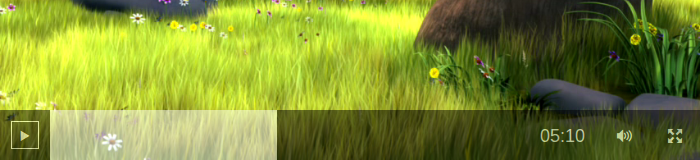
\includegraphics[width=\textwidth]{accessibility/button}
		\caption{The play button when focused. In this state, pressing the space bar plays or pauses the video.}
		\label{Figure:Accessibility/Screenshots/Button}
	\end{subfigure}
	\begin{subfigure}[]{\textwidth}
		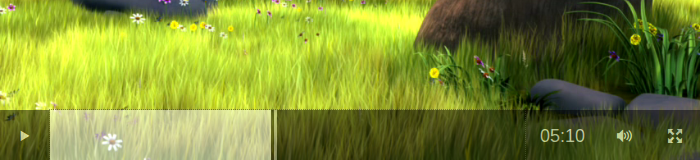
\includegraphics[width=\textwidth]{accessibility/scrub-bar}
		\caption{The scrub bar when focused. In this state, pressing the left or right arrow keys skips backwards or forwards in the video.}
		\label{Figure:Accessibility/Screenshots/ScrubBar}
	\end{subfigure}
	\begin{subfigure}[]{\textwidth}
		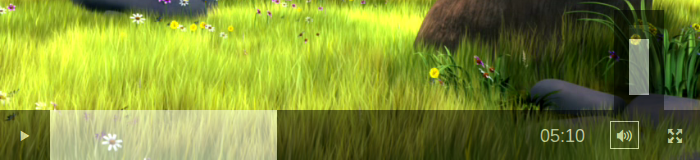
\includegraphics[width=\textwidth]{accessibility/volume}
		\caption{The mute button and volume control when the mute button is focused. In this state, pressing the space bar toggles mute, and the up and down arrow keys change the volume.}
		\label{Figure:Accessibility/Screenshots/Volume}
	\end{subfigure}
	\caption{Screenshots of the accessibility improvements made to Videogular's HTML controls.}
	\label{Figure:Accessibility/Screenshots}
\end{figure}

\subsection{Conclusions} 
This solution is not completely clicker-accessible, but could be made so by introducing buttons to skip forwards or backwards, and to raise or lower the volume. It is a significant improvement on the original state, as keyboard users can now use the player. The improvements were submitted to the \gls{Videogular} project\footnote{\url{https://github.com/2fdevs/videogular/pull/108}}, and are now part of \gls{Videogular} 0.6.1.


\section{Compatibility} 
\label{Section:Compatibility}

One of the main focuses of this part of the project was to make sure the application was compatible with a range of platforms, operating systems and devices. The first challenge was to ensure that the player and overlay displayed correctly at a variety of resolutions and screen/window sizes. 

Apple iPhones provided a problem as iOS forced the video to be played in fullscreen mode. This is a design choice and there is no way to play the video inline, directives to do this are ignored by the browser.

This meant that the video paused at the correct time but as the video is in the native player the overlay was not visible unless the player is quit. There is no way of notifying the user that this needs to be done. A possible solution involves telling the user to quit out of the video when it is paused so they may answer the question. However this is not very user friendly. iOS software on Apple tablets however does not have this limitation and the video will play inline correctly as the device is large enough.

Android phones correctly interpret the inline directive and will properly play this. This ensures that the overlay is correctly applied and usable. This has been the primary focus on testing on mobile devices as it represents a very large portion of the market.

The overlay which displays the questions that the user is asked appears above the video and obstructs the view of the video. Placing the overlay in the middle of the screen requires a large amount of \gls{CSS} to correctly locate it on the screen for mobile and smaller sized devices. There are still some issues with the popup location on some mobile devices because the browser reports one screen size and uses another. Until these devices are compliant with the specification it is time consuming to write code to fix each individual case.

The best user experience with this application is using it on a desktop that has an updated browser. This will definitely work and display as intended. As the screen size of the device gets smaller the user experience is significantly reduced as the video and poll overlay will be much smaller than recommended. To support a number of browsers and operating systems a range of video formats are supplied to the \gls{Videogular} plugin so that the browser may pick one that can be played.

\section{Scrub Bar Extensions} 
\label{Section:Scrub Bar Extensions}

\gls{Videogular} has been designed and implemented in such a way as to allow for directive-based plugins to be developed to extend its functionality. When using the \gls{Videogular} Controls (vgControls) the native browser controls are replaced with an HTML based interface. It is this interface we have improved the accessibility of, and it is the scrub bar within this interface we have created plugins for.

The team behind \gls{Videogular}, 2fdev, are actively seeking members of the community to develop new plugins for their system, and as such are willing to discuss future plugins and their architectural design.

\subsection{Videogular Cuepoints - vgCuepoints}
\label{Subsection:vgCuepoints}
\gls{Videogular} Cuepoints is a \gls{Videogular} plugin for displaying `cuepoints', marks on the scrub bar which can be positioned at a particular time. For example, cuepoints could be used to indicate the start of a section in the video, or a time when a pop-up will appear.

\subsubsection{Design and Implementation}

\subsubsection{Conclusions} 

\subsection{Videogular Heatmaps - vgHeatmap}
\gls{Videogular} Heatmaps is a \gls{Videogular} plugin for giving areas of the scrub bar different colours. In our examples this is used to give a visual representation of the number of times each section of the video has been watched.

\subsubsection{Design and Implementation}
An early design decision was to use \gls{CSS} to colour the sections as this would allow different colours to be specified (see \cref{Req:Use of colour}). This also would allow developers to develop their own colour schemes with meanings if they desired.

Sections and colours can be specified in a \texttt{config} object which is given as a parameter when the heat map is used. 

The schema for defining the configuration parameters was made consistent with vgCuepoints (see \autoref{Subsection:vgCuepoints}) to improve usability.

One problem found during implementation was that the heat map cannot be displayed before the video has begun playing. This is due to \gls{Videogular} not setting the video length variable until it begins playing, thus this variable cannot be used to calculate the widths of the sections until it is set. This was accepted as the colouring does not have any context for a user until they have watched the video.

\subsubsection{Conclusions} 
